\documentclass[11pt,a4paper]{article}
\usepackage[margin=2.2cm]{geometry}
\usepackage{amsmath,amssymb,bm}
\usepackage{graphicx,float,booktabs,caption,subcaption}
\usepackage{xcolor}
\usepackage{listings}
\usepackage{tikz}
\usetikzlibrary{shapes.geometric,arrows.meta,positioning,calc}
\usepackage[colorlinks=true,linkcolor=blue!50!black,urlcolor=blue!50!black,citecolor=blue!50!black]{hyperref}
\usepackage{fancyhdr}
\pagestyle{fancy}\fancyhf{}\lhead{\small Karthick J (OE23S018), IIT Madras}\rhead{\small\leftmark}\cfoot{\thepage}
\definecolor{codebg}{rgb}{0.97,0.97,0.97}
\lstset{basicstyle=\ttfamily\scriptsize,backgroundcolor=\color{codebg},frame=single,breaklines=true,
 keywordstyle=\color{blue!60!black}\bfseries,commentstyle=\color{green!40!black},stringstyle=\color{red!50!black},
 numbers=left,numberstyle=\tiny\color{gray},showstringspaces=false,tabsize=4,columns=fullflexible,
 literate={²}{{$^2$}}1 {³}{{$^3$}}1 {°}{{$^\circ$}}1 {Δ}{{$\Delta$}}1 {ρ}{{$\rho$}}1 {μ}{{$\mu$}}1 {ω}{{$\omega$}}1 {ψ}{{$\psi$}}1 {α}{{$\alpha$}}1 {ν}{{$\nu$}}1 {τ}{{$\tau$}}1 {–}{{-}}1 {—}{{-}}1 {’}{{'}}1 {“}{{"}}1 {”}{{"}}1 {→}{{$\to$}}1 {≤}{{$\le$}}1 {≥}{{$\ge$}}1 {×}{{$\times$}}1 {±}{{$\pm$}}1 {·}{{$\cdot$}}1 {∂}{{$\partial$}}1 {∇}{{$\nabla$}}1 {γ}{{$\gamma$}}1 {ε}{{$\varepsilon$}}1 {μ}{{$\mu$}}1 {├}{{+}}1 {─}{{-}}1 {│}{{|}}1 {▶}{{>}}1 {▼}{{v}}1 {┌}{{+}}1 {┐}{{+}}1 {└}{{+}}1 {┘}{{+}}1 {┬}{{+}}1 {┴}{{+}}1}
\tikzset{
 startstop/.style={rectangle,rounded corners=6pt,minimum width=3.2cm,minimum height=0.8cm,text centered,draw=black,fill=red!12,font=\small},
 process/.style={rectangle,minimum width=4.6cm,minimum height=0.8cm,text centered,text width=5.6cm,draw=black,fill=blue!8,font=\small},
 decision/.style={diamond,aspect=2.6,text centered,text width=3.2cm,draw=black,fill=green!12,font=\small,inner sep=1pt},
 io/.style={trapezium,trapezium left angle=72,trapezium right angle=108,minimum width=3.6cm,minimum height=0.8cm,text centered,text width=4.6cm,draw=black,fill=orange!15,font=\small},
 arrow/.style={thick,-{Stealth[length=2.5mm]}}}
\setlength{\parskip}{4pt}\setlength{\parindent}{0pt}

\title{\textbf{1-D Transient Heat Conduction in a Flat Plate}\\[2pt]\large Explicit (FTCS) Finite-Difference Solution in C\\[2pt]\normalsize Course Project 7 -- AM5630 Foundation of Computational Fluid Dynamics (Jul--Nov 2024)}
\author{Karthick J (OE23S018)\\Department of Ocean Engineering, IIT Madras\\Faculty: Prof.\ Arul Prakash}
\date{Revised report, October 2026}
\begin{document}\maketitle
\begin{abstract}
The transient temperature field in a one-dimensional plate with a sudden step in wall temperature is computed with the explicit forward-time / central-space (FTCS) finite-difference scheme implemented in C. The solution is obtained for three time steps ($\Delta t=0.1,\,0.01,\,0.001$~s) and compared with the exact Fourier-series solution. The original code was reviewed; three defects (an integer-typed length, a one-step offset in the time labels, and insufficient output precision) were corrected in the C code, and an in-place update in the MATLAB plotting script that silently turned the explicit scheme into a Gauss--Seidel-type sweep was fixed. The corrected solver reproduces the analytical profile to within $5.3\times10^{-3}$ (maximum absolute error) at $t=10$~s, the error being dominated by the spatial truncation term $\mathcal{O}(\Delta x^2)$. A run at $\gamma=0.625$ confirms the von Neumann stability limit $\gamma\le 1/2$.
\end{abstract}
\tableofcontents\newpage

\section{Problem definition}
A plate of length $L=100$ (length units of the original code; written as cm) is initially at $T=0$. At $t=0^+$ the left face is raised to $T=1$ and the right face is held at $T=0$. Heat transfer is by conduction only, with constant diffusivity $\alpha=1$.
\begin{align}
\frac{\partial T}{\partial t} &= \alpha\,\frac{\partial^2 T}{\partial x^2}, && 0<x<L,\; t>0, \label{eq:gov}\\
T(x,0)&=0, \qquad T(0,t)=1, \qquad T(L,t)=0. \nonumber
\end{align}
(The original report titled the problem ``heat convection''; Eq.~\eqref{eq:gov} is the pure-diffusion, i.e.\ conduction, equation and that is what the code solves.)

\section{Numerical formulation}
\subsection{Discretisation}
The domain is divided into $N_x=51$ nodes, $\Delta x=L/(N_x-1)=2$. Forward differencing in time and second-order central differencing in space give
\begin{equation}
T_i^{n+1} = \gamma\,T_{i-1}^{n} + (1-2\gamma)\,T_i^{n} + \gamma\,T_{i+1}^{n}, \qquad \gamma=\frac{\alpha\,\Delta t}{\Delta x^2}, \label{eq:ftcs}
\end{equation}
with local truncation error $\mathcal{O}(\Delta t,\Delta x^2)$. All right-hand-side values belong to the \emph{old} time level $n$, which is what makes the scheme explicit.

\subsection{Stability}
Substituting a Fourier mode $T_i^n=G^n e^{\mathrm{i}k i\Delta x}$ into \eqref{eq:ftcs} gives the amplification factor $G=1-4\gamma\sin^2(k\Delta x/2)$. $|G|\le1$ for all wavenumbers requires
\begin{equation}\gamma=\frac{\alpha\Delta t}{\Delta x^2}\le\frac12 .\end{equation}
For $\Delta x=2$ the limit is $\Delta t\le 2$~s; the three production runs use $\gamma=2.5\times10^{-2},\,2.5\times10^{-3},\,2.5\times10^{-4}$, and an extra run at $\Delta t=2.5$~s ($\gamma=0.625$) is used to demonstrate the instability.

\subsection{Modified equation and consistency}
Expanding \eqref{eq:ftcs} in Taylor series about $(x_i,t^n)$ and eliminating the time derivatives with the PDE gives the equation that the scheme actually solves,
\begin{equation}
\frac{\partial T}{\partial t}=\alpha\frac{\partial^2T}{\partial x^2}+\frac{\alpha\Delta x^2}{12}\,(1-6\gamma)\,\frac{\partial^4T}{\partial x^4}+\mathcal{O}(\Delta x^4).
\end{equation}
The scheme is consistent and second-order in space at fixed $\gamma$; the leading error term changes sign at $\gamma=1/6$. Equivalently, the per-step decay of a Fourier mode, $\ln G=-\gamma\theta^2+\gamma\theta^4(1-6\gamma)/12+\dots$ with $\theta=k\Delta x$, matches the exact $-\gamma\theta^2$ to fourth order only when $\gamma=1/6$.

\subsection{Analytical reference solution}
Separation of variables gives the exact solution used for verification:
\begin{equation}
T(x,t)=1-\frac{x}{L}-\frac{2}{\pi}\sum_{n=1}^{\infty}\frac{1}{n}\sin\!\Big(\frac{n\pi x}{L}\Big)\exp\!\Big(-\frac{n^2\pi^2\alpha t}{L^2}\Big),
\end{equation}
evaluated with 400 terms.

\subsection{Algorithm and flowchart}
\begin{figure}[H]\centering
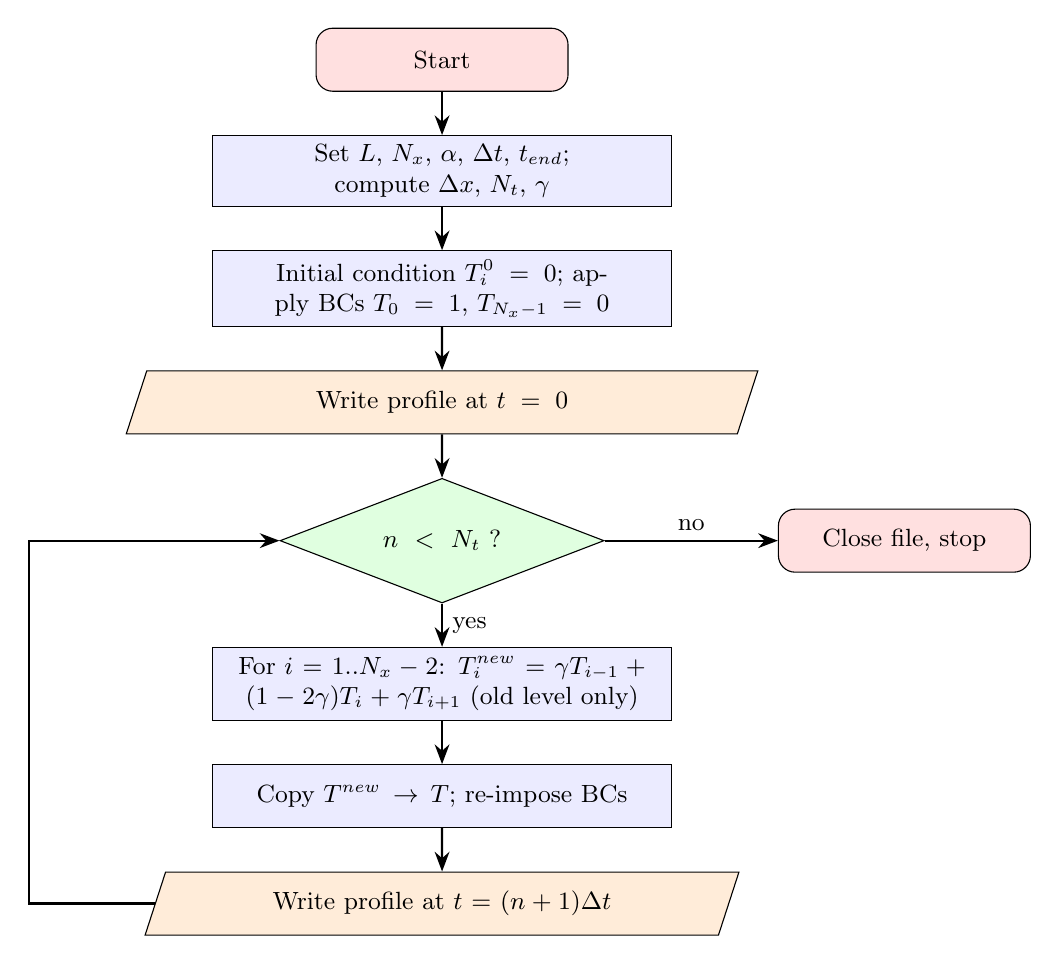
\begin{tikzpicture}[node distance=0.55cm]
\node (s) [startstop] {Start};
\node (i) [process, below=of s] {Set $L$, $N_x$, $\alpha$, $\Delta t$, $t_{end}$; compute $\Delta x$, $N_t$, $\gamma$};
\node (ic)[process, below=of i] {Initial condition $T_i^0=0$; apply BCs $T_0=1$, $T_{N_x-1}=0$};
\node (w0)[io, below=of ic] {Write profile at $t=0$};
\node (l) [decision, below=of w0] {$n<N_t$ ?};
\node (u) [process, below=of l] {For $i=1..N_x-2$: $T_i^{new}=\gamma T_{i-1}+(1-2\gamma)T_i+\gamma T_{i+1}$ (old level only)};
\node (c) [process, below=of u] {Copy $T^{new}\to T$; re-impose BCs};
\node (w) [io, below=of c] {Write profile at $t=(n+1)\Delta t$};
\node (e) [startstop, right=2.2cm of l] {Close file, stop};
\draw[arrow](s)--(i); \draw[arrow](i)--(ic); \draw[arrow](ic)--(w0); \draw[arrow](w0)--(l);
\draw[arrow](l)--node[right,font=\small]{yes}(u); \draw[arrow](u)--(c); \draw[arrow](c)--(w);
\draw[arrow](w.west)--++(-1.6,0)|-(l.west); \draw[arrow](l)--node[above,font=\small]{no}(e);
\end{tikzpicture}
\caption{Flowchart of the explicit FTCS solver (\texttt{code/assignment\_1.c}).}\end{figure}

\section{Code review and corrections}
The original code was kept unchanged except for the defects below (every change is marked \texttt{[FIX]} in the source; the untouched originals are in \texttt{original/}).
\begin{table}[H]\centering\small
\begin{tabular}{p{0.5cm}p{3.4cm}p{5.4cm}p{4.6cm}}\toprule
\# & Location & Problem & Correction\\\midrule
1 & C: \texttt{int L = 100;} & $\Delta x=L/(N_x-1)$ is computed in integer arithmetic. It happens to be exact for $L=100$, but the version in the submitted report ($L=1$) gives $\Delta x=0$ and $\gamma=\infty$. & Declared \texttt{double L = 100.0}.\\
2 & C: time loop & The loop started at $j=0$ and updated the field \emph{before} writing it under the label $t=j\Delta t$, so every stored profile was one step later than its label and $t=0$ was never written. & Write the initial condition first; loop $j=1..N_t$ and label the state after $j$ steps $t=j\Delta t$.\\
3 & C: output & Profiles were written with 2 decimals, hiding the early-time solution ($T<0.005$ printed as 0.00). & 6 decimals.\\
4 & MATLAB: interior update & \texttt{grid(i)} was overwritten in place, so \texttt{grid(i-1)} on the right-hand side was already the new value. This is a Gauss--Seidel-type sweep, not Eq.~\eqref{eq:ftcs}; the same one-step label offset (fix 2) was also present. The plots in the original report came from this script. & Use a copy \texttt{Told} of the previous level on the right-hand side.\\\bottomrule
\end{tabular}\caption{Defects found and corrected.}\end{table}
The numerical method, grid, parameters and output format were not otherwise changed. The console printing of every node at every step was left in place; \texttt{run.sh} redirects it to \texttt{/dev/null}.

\section{Results}
\subsection{Temperature profiles}
\begin{figure}[H]\centering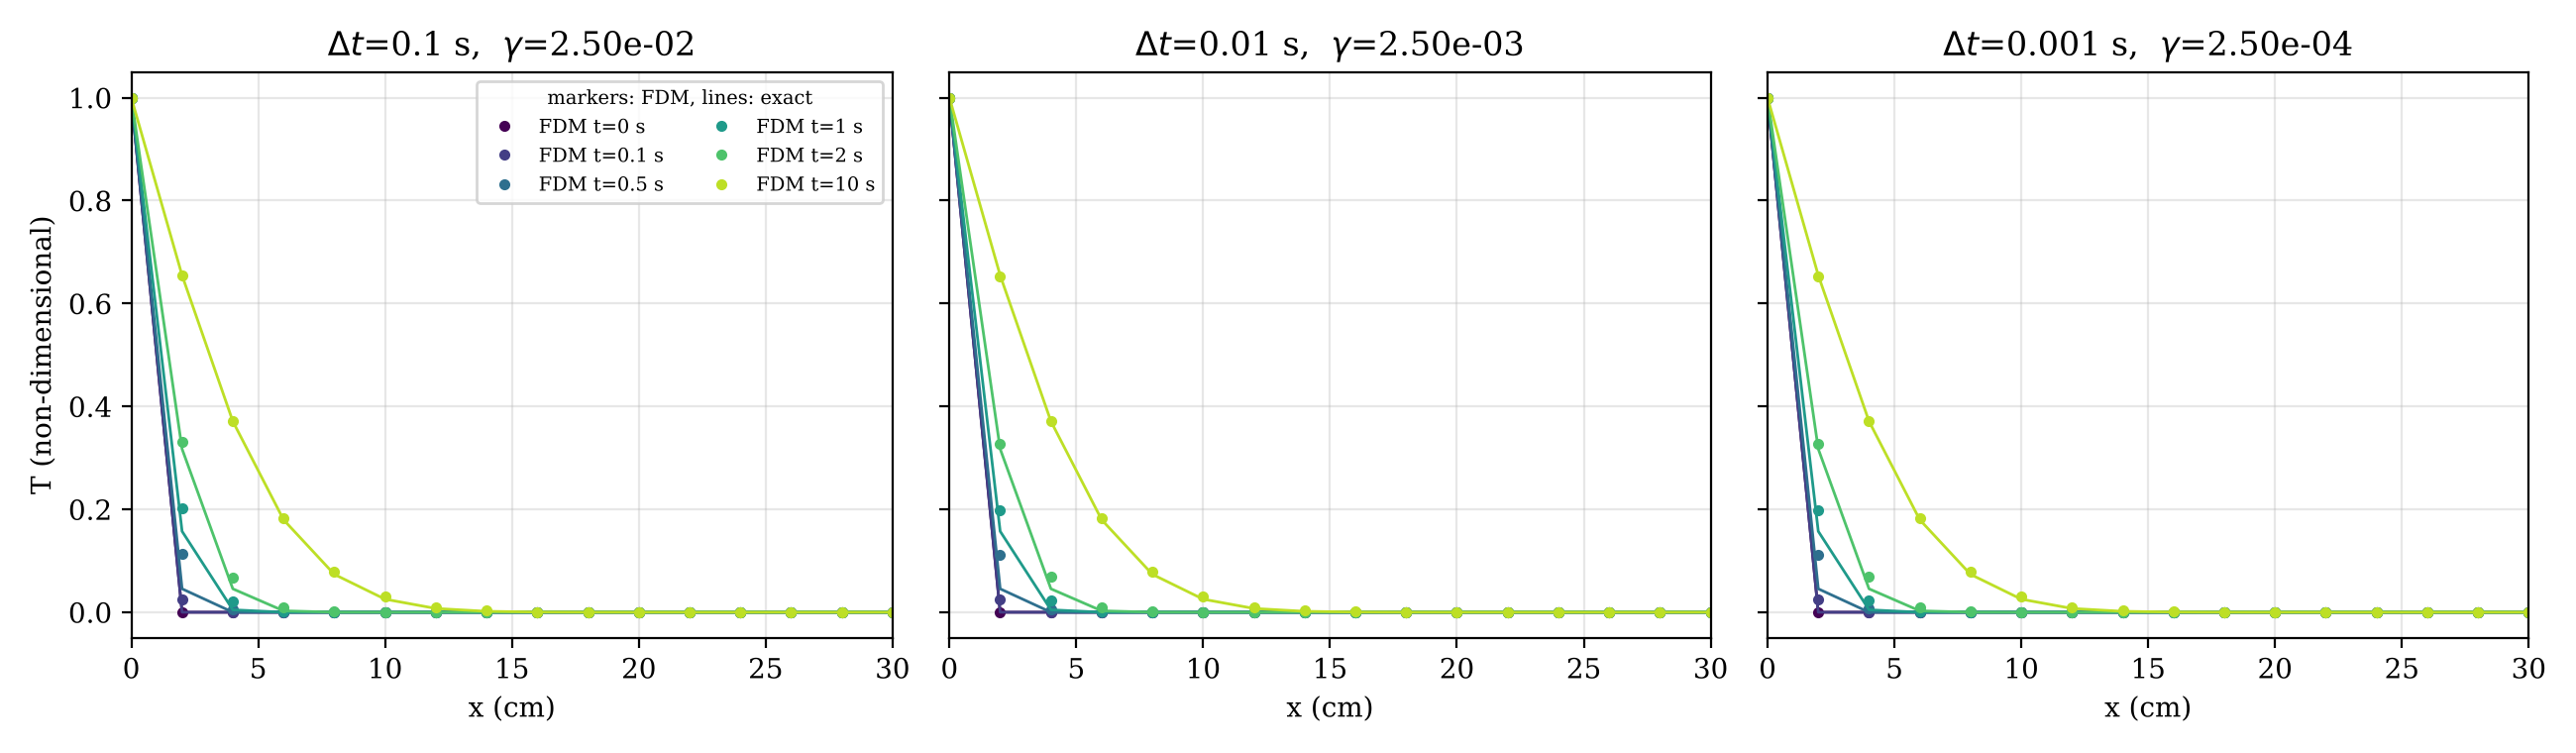
\includegraphics[width=\textwidth]{../results/fig1_profiles_vs_exact.png}
\caption{FDM profiles (markers) against the exact solution (lines) at $t=0,0.1,0.5,1,2,10$~s for the three time steps. Only $0\le x\le30$ is shown; the field is zero beyond.}\end{figure}
The thermal front penetrates a distance of order $\sqrt{\alpha t}$ ($\approx3.2$ at $t=10$~s), so at the final time the disturbance has reached only $\sim15\%$ of the plate and the right boundary plays no role. The three time steps give visually identical profiles, and all agree with the exact solution; at $x=2$, $t=10$~s the FDM gives $T=0.6525$ against $T=0.6547$ exactly.

\begin{figure}[H]\centering
\begin{subfigure}{0.48\textwidth}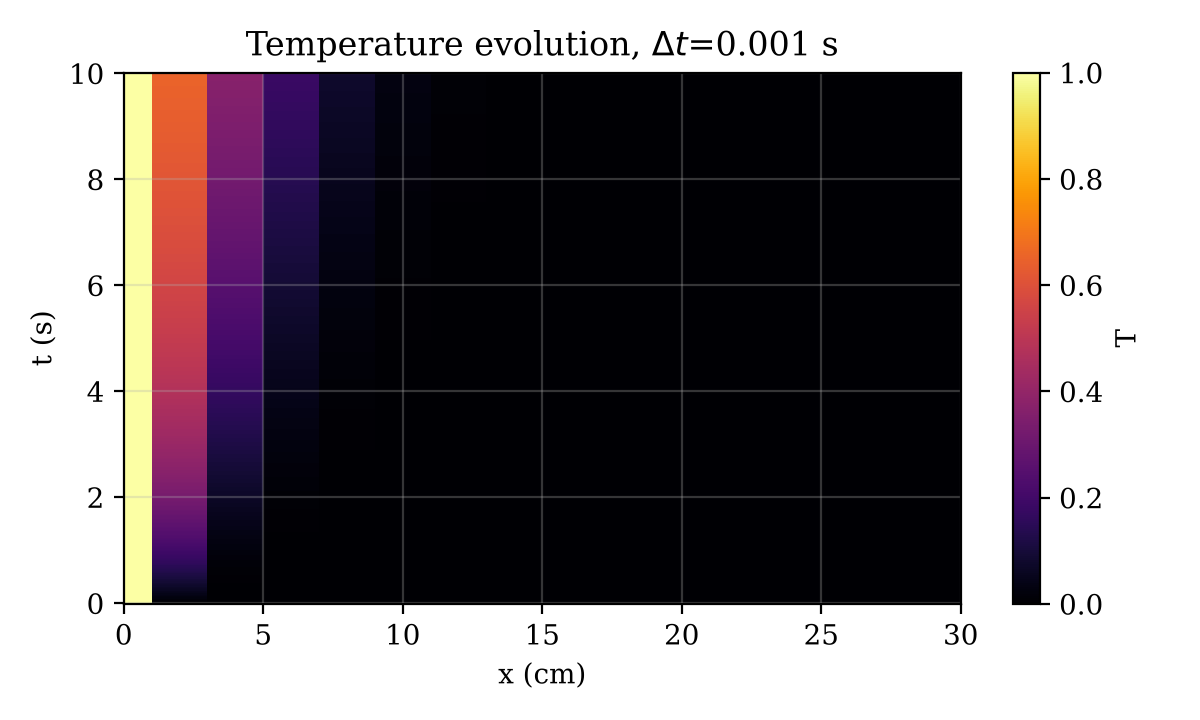
\includegraphics[width=\textwidth]{../results/fig3_space_time.png}\caption{Space--time map, $\Delta t=0.001$~s.}\end{subfigure}\hfill
\begin{subfigure}{0.48\textwidth}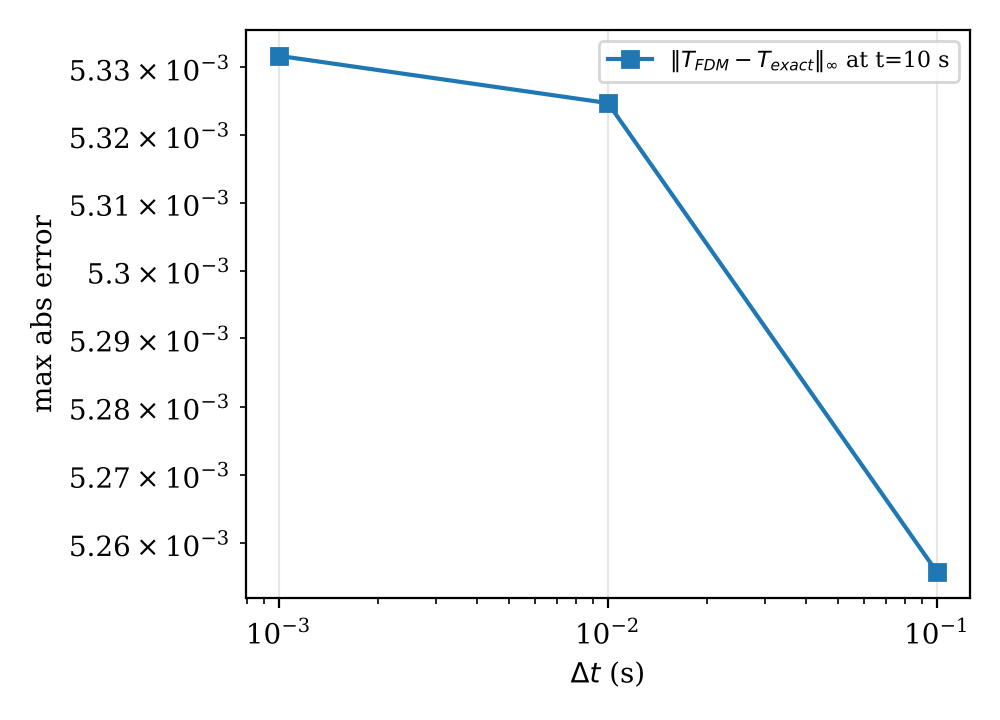
\includegraphics[width=\textwidth]{../results/fig2_error_vs_dt.png}\caption{Maximum error at $t=10$~s.}\end{subfigure}
\caption{Evolution of the field and dependence of the error on $\Delta t$.}\end{figure}

\subsection{Accuracy}
\begin{table}[H]\centering\begin{tabular}{cccc}\toprule
$\Delta t$ (s) & $\gamma$ & $N_t$ & $\max|T_{FDM}-T_{exact}|$ at $t=10$~s\\\midrule
0.1 & $2.5\times10^{-2}$ & 100 & $5.26\times10^{-3}$\\
0.01 & $2.5\times10^{-3}$ & 1\,000 & $5.33\times10^{-3}$\\
0.001 & $2.5\times10^{-4}$ & 10\,000 & $5.33\times10^{-3}$\\\bottomrule\end{tabular}
\caption{Error against the exact solution.}\end{table}
The error is essentially independent of $\Delta t$: because $\gamma\ll1/2$ in all runs the temporal error $\mathcal{O}(\Delta t)$ is negligible and the remaining error is the spatial truncation term $\mathcal{O}(\Delta x^2)$ with $\Delta x=2$. Refining the grid, not the time step, is the way to improve accuracy for this set-up; the largest stable time step ($\gamma\to1/2$) would therefore be the most economical choice.

\subsection{Accuracy study: grid refinement and the effect of $\gamma$}
Two additional sets of runs of the same program (only \texttt{CX}, \texttt{dt} and the end time substituted, \texttt{run.sh}) quantify the accuracy.
\begin{figure}[H]\centering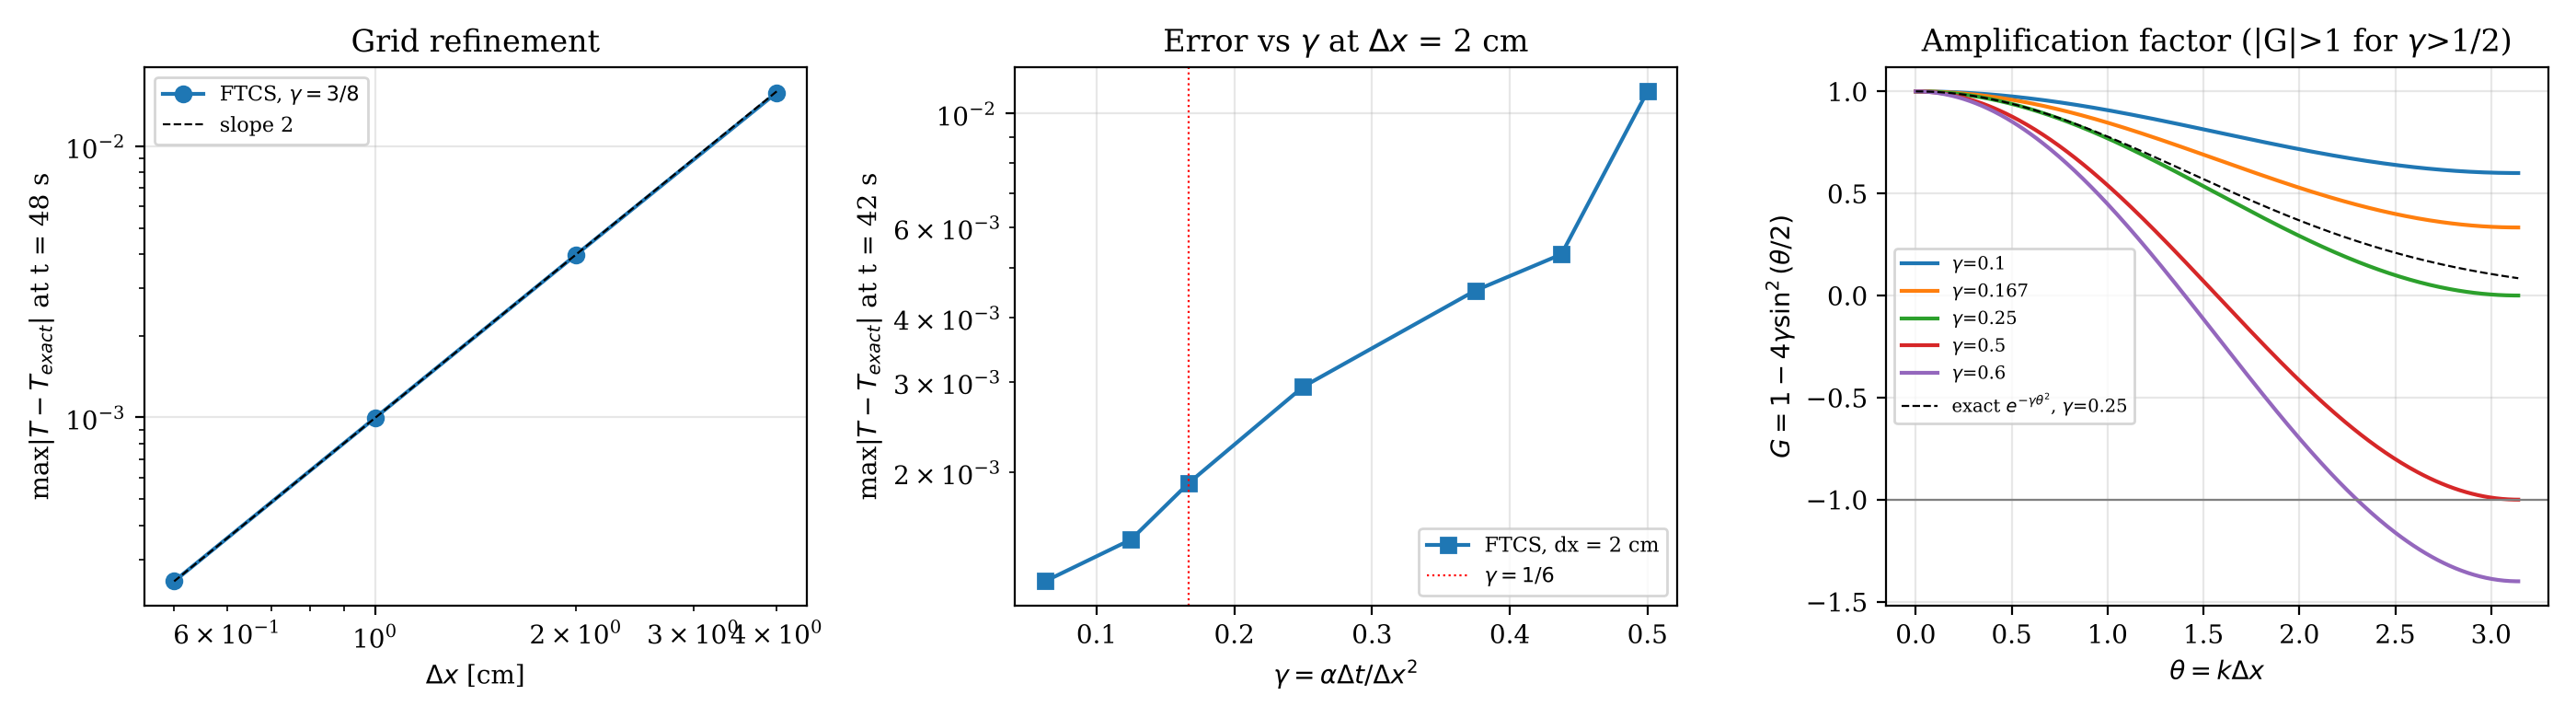
\includegraphics[width=\textwidth]{../results/fig6_accuracy_study.png}
\caption{Left: maximum error at $t=48$~s for $\Delta x=4,2,1,0.5$ cm at fixed $\gamma=3/8$. Centre: error at $t=42$~s against $\gamma$ for $\Delta x=2$ cm. Right: amplification factor of FTCS against the exact decay $e^{-\gamma\theta^2}$.}\end{figure}
\begin{table}[H]\centering\small\begin{tabular}{cccc}\toprule
$N_x$ & $\Delta x$ [cm] & $\max|T-T_{exact}|$, $t=48$ s & observed order\\\midrule
26 & 4 & $1.576\times10^{-2}$ & --\\
51 & 2 & $3.973\times10^{-3}$ & 1.99\\
101 & 1 & $9.958\times10^{-4}$ & 2.00\\
201 & 0.5 & $2.488\times10^{-4}$ & 2.00\\\bottomrule\end{tabular}
\caption{Grid refinement at constant $\gamma$ ($\Delta t\propto\Delta x^2$; \texttt{results/accuracy\_study.txt}).}\end{table}
The observed order is 2.00, as predicted by the modified equation. At fixed $\Delta x=2$ cm the error grows from $1.2\times10^{-3}$ at $\gamma=0.0625$ to $5.3\times10^{-3}$ at $\gamma=0.44$ and doubles again at the stability limit $\gamma=1/2$, where the highest mode is no longer damped ($G(\pi)=-1$). The cancellation at $\gamma=1/6$ predicted for smooth solutions does not appear as a minimum here, because the error at this resolution is dominated by the representation of the discontinuous start-up (the boundary jumps from 0 to 1 at $t=0$), which no choice of $\gamma$ removes. Practically, $\gamma\approx0.1$--$0.25$ balances accuracy and cost.

\subsection{Comparison with the original plots}
\begin{figure}[H]\centering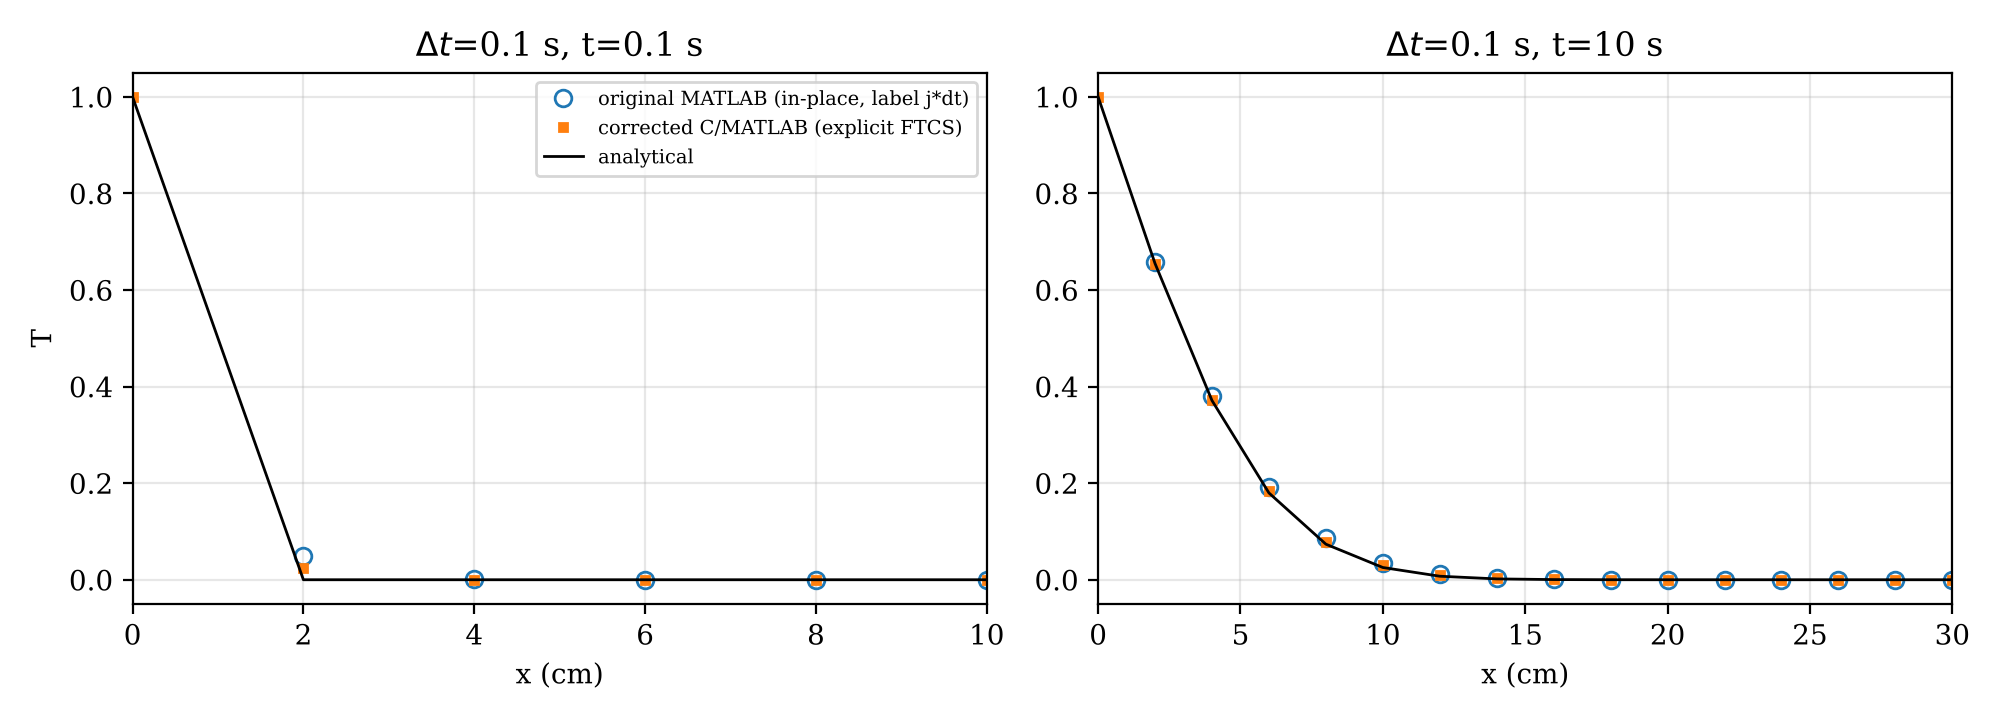
\includegraphics[width=\textwidth]{../results/fig4_old_vs_corrected.png}
\caption{Original MATLAB result (in-place sweep, one-step label offset) versus the corrected explicit scheme and the exact solution, $\Delta t=0.1$~s.}\end{figure}
At $t=10$~s the original and corrected results almost coincide, which is why the original plots looked correct. At early times the difference is visible: at $t=0.1$~s the original plot shows $T(2)=0.0487$ (two in-place updates) whereas the explicit scheme gives $0.025$ after one step. The original plots are kept in \texttt{original/Original\_Report\_Plots.pdf}.

\subsection{Stability demonstration}
\begin{figure}[H]\centering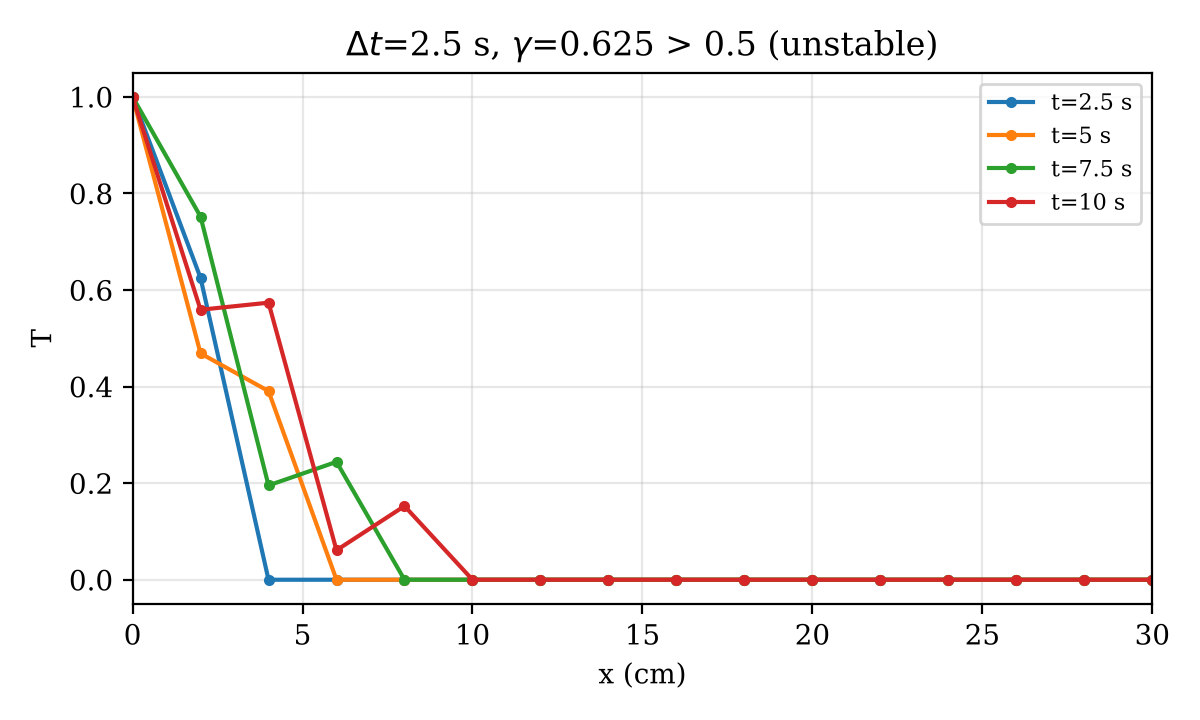
\includegraphics[width=0.62\textwidth]{../results/fig5_stability_gamma_gt_half.png}
\caption{$\Delta t=2.5$~s ($\gamma=0.625$): the node-to-node (odd--even) oscillation characteristic of $|G|>1$ appears immediately.}\end{figure}

\section{Conclusions}
\begin{itemize}
\item The explicit FTCS scheme implemented in C reproduces the exact transient conduction solution to within $5.3\times10^{-3}$ at $t=10$~s for all three time steps.
\item With $\gamma\ll 1/2$ the error is controlled by $\Delta x$; the time-step study shows temporal convergence is already saturated.
\item The stability bound $\gamma\le1/2$ was confirmed numerically, and a four-grid refinement study confirmed second-order spatial convergence (observed order 2.00), in agreement with the modified-equation analysis.
\item Four implementation defects were corrected without changing the method; the most significant was the in-place update in the MATLAB script, which had changed the scheme that produced the original plots.
\end{itemize}

\section*{Reproducing the results}
\texttt{bash run.sh} compiles \texttt{code/assignment\_1.c} for each $\Delta t$, runs it, and calls \texttt{code/plot\_results.py} (Python 3, NumPy, Matplotlib). It then runs the accuracy studies (\texttt{code/study.py}). Outputs go to \texttt{results/}.

\appendix\section{Source code (corrected)}
\lstinputlisting[language=C]{../code/assignment_1.c}
\end{document}
